\section{Results}
\label{sec:analysis}
\label{sec:results}
We first report study selection and the validation of screening and extraction, then the characteristics of the 120 included studies: publication trends, modalities and territories, tasks and architectures, temporal modeling, venues, reported performance and reporting quality.

\subsection{Study Selection and Review Corpus}
The search identified 5,829 records (PubMed/\allowbreak MEDLINE 4,071; Semantic Scholar 1,758). After removing 765 duplicates, we screened 5,064 records (Figure~\ref{fig:prisma}). The LLM labelled 134 as eligible and excluded 4,930: 4,831 failed at least one inclusion criterion and 99 met an exclusion criterion (E1: 3, E2: 95, E3: 1). Cochran's formula set the validation sample at 357 of the 4,930 exclusions, so the reviewers screened 491 records.

The two reviewers agreed on 487 of the 491 records (99.2\%; Cohen's $\kappa=0.978$, 95\% CI 0.957--0.999). Each reviewer included two records the other excluded; in all four cases the consensus followed the interventional radiologist. Against this gold standard, the pipeline was correct for 120 of its 134 INCLUDE decisions (89.6\%; 95\% Wilson CI 83.2--93.7\%) and for 355 of the 357 sampled EXCLUDE decisions (99.4\%; 98.0--99.8\%). Weighted by stratum size, overall agreement was 99.2\%, and precision, recall and F1 for the INCLUDE class were 0.90, 0.81 and 0.85 ($\kappa=0.85$). The recall estimate rests on two missed studies, both of which failed criterion I2, and is imprecise (Section~\ref{sec:limitations}).

Following the gold standard, we excluded 14 LLM-eligible records and added the 2 eligible records found among the exclusions, giving 122 eligible studies; Figure~\ref{fig:prisma} therefore lists 4,829 rather than 4,831 LLM inclusion failures. Full text could not be retrieved for 2 of them (R4468, R4475), so the review corpus comprises 120 studies. Three are earlier versions (preprint or conference paper) of another included study and are counted separately. All 491 screening decisions are listed in Supplementary Table~S1.

The extraction audit covered 6 of the 120 studies (5\%) and 444 values: per study, 18 study-level fields, the status of the 12 research gaps and the 44 CLAIM 2024 items. The reviewer judged 431 values correct (97.1\%; 95.1--98.3\%), 13 incorrect and none unclear. All errors were interpretive (the task labels of one study, gap statuses and individual CLAIM items); descriptive fields such as modality, territory, cohort size, temporal category and validation design were correct in all six studies. Per-gap counts and item-level CLAIM percentages should therefore be read as approximate.

\begin{figure*}[htbp]
  \centering
  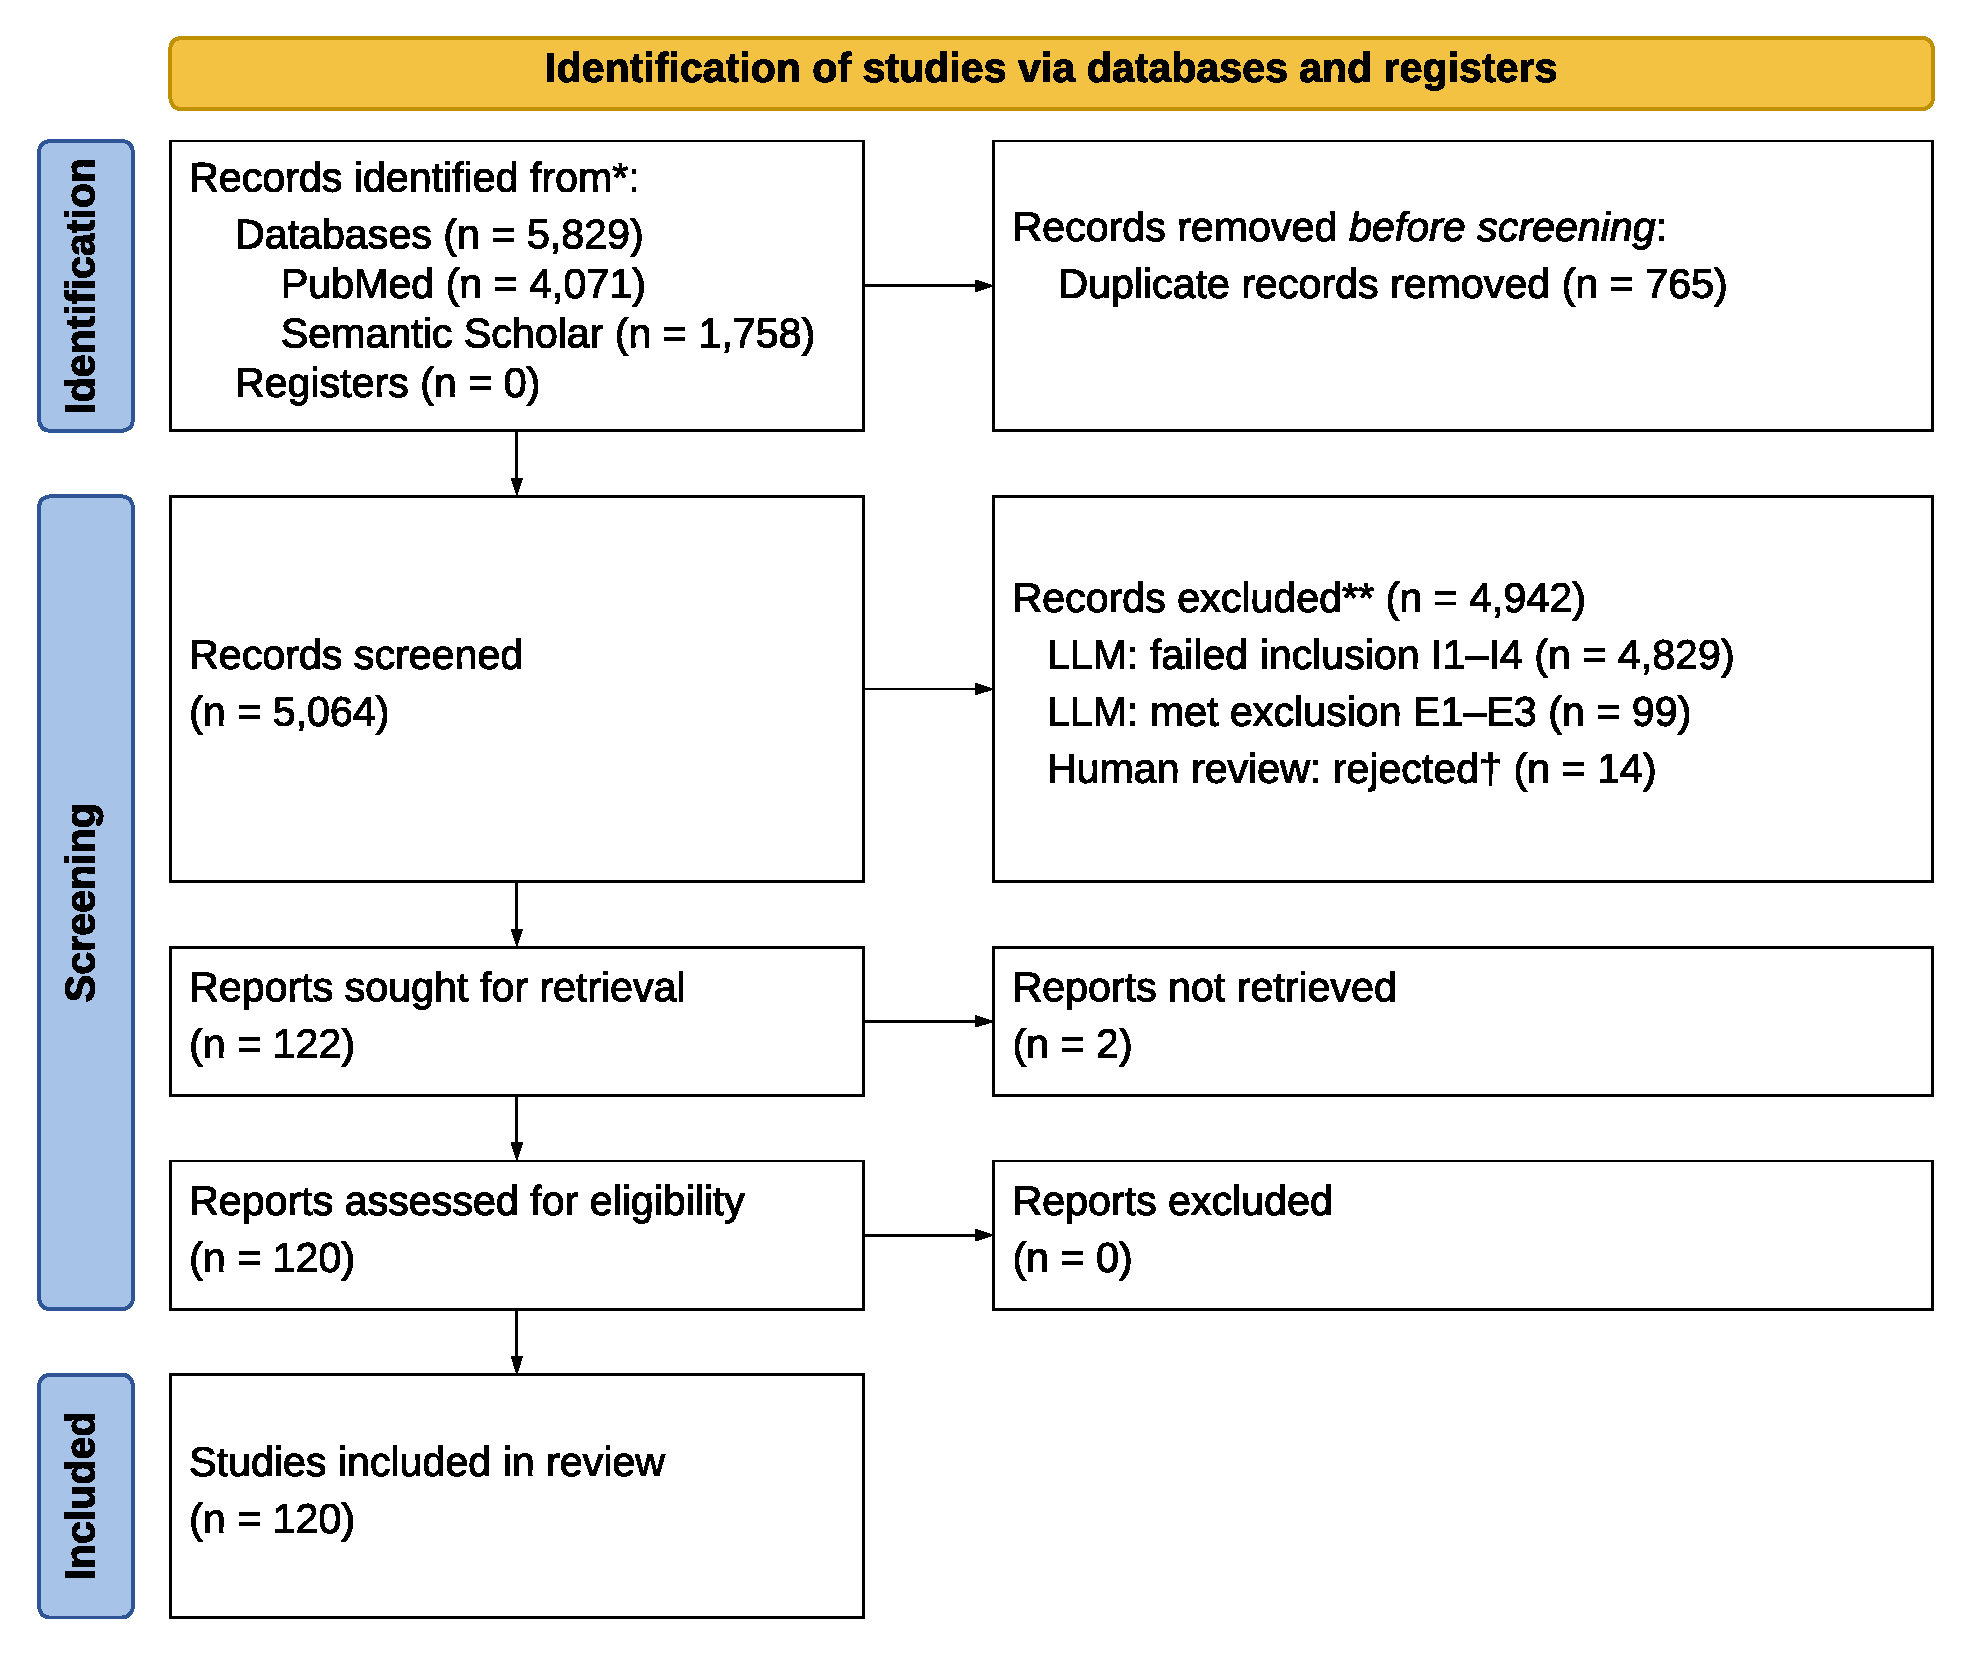
\includegraphics[width=\textwidth]{figs/prisma.pdf}
  \caption{PRISMA 2020 flow diagram summarizing the study identification, screening, eligibility assessment, and inclusion process used in this systematic review}
  \label{fig:prisma}
\end{figure*}



\subsection{Publication Trends}
\label{subsec:trends}
\begin{figure}[]
\centering
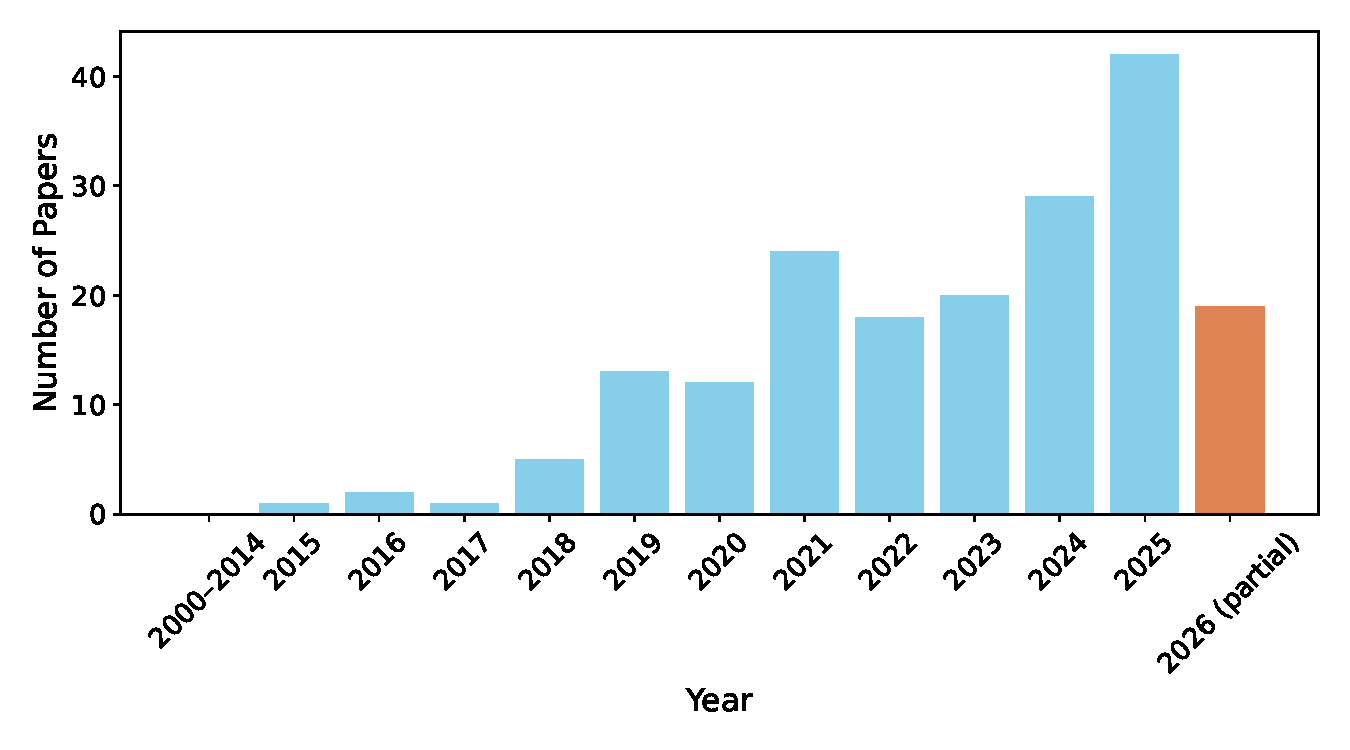
\includegraphics[width=1\linewidth]{figs/temporal_trends.pdf}
\caption{Included studies by publication year. The 2026 bar covers a partial year.}
\label{fig:temporal_trends}
\end{figure}

No included study predates 2018, and only five appeared in 2018--2019 (Figure~\ref{fig:temporal_trends}). Output rose sharply after 2020 and stayed high through 2025; the partial year 2026 already exceeds several earlier full years. Transformer-based temporal models came late: all ten in the corpus were published from 2023 onward.

\vspace{0.25cm}
\begin{mdframed}[linewidth=0.5pt, linecolor=black, backgroundcolor=blue!10]
\textbf{Finding 1.} The field is young and still growing: 78\% of studies (94/120) were published from 2022 to 2026.
\end{mdframed}
\vspace{0.25cm}

\subsection{Imaging Modalities and Anatomical Coverage}
\label{subsec:modality_anatomy}
\begin{figure}[]
\centering
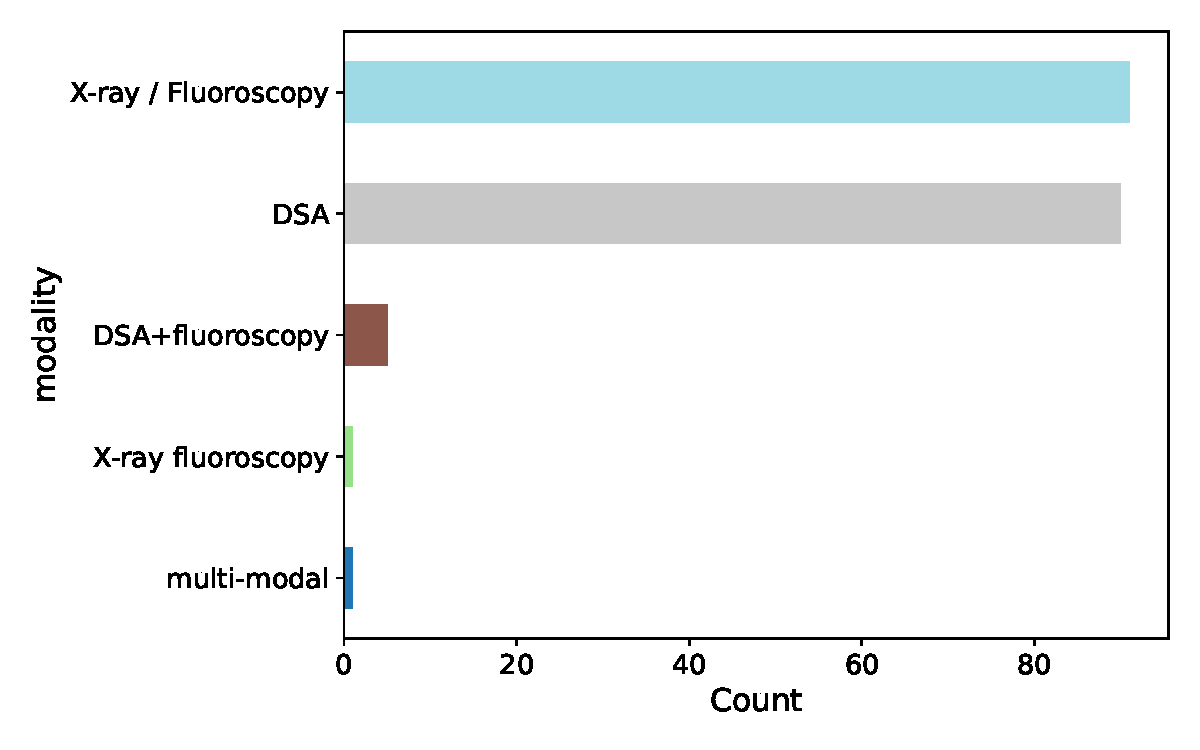
\includegraphics[width=1\linewidth]{figs/modality_distribution.pdf}
\caption{Imaging modality distribution across included studies.}
\label{fig:modality_distribution}
\end{figure}
\begin{figure}[]
\centering
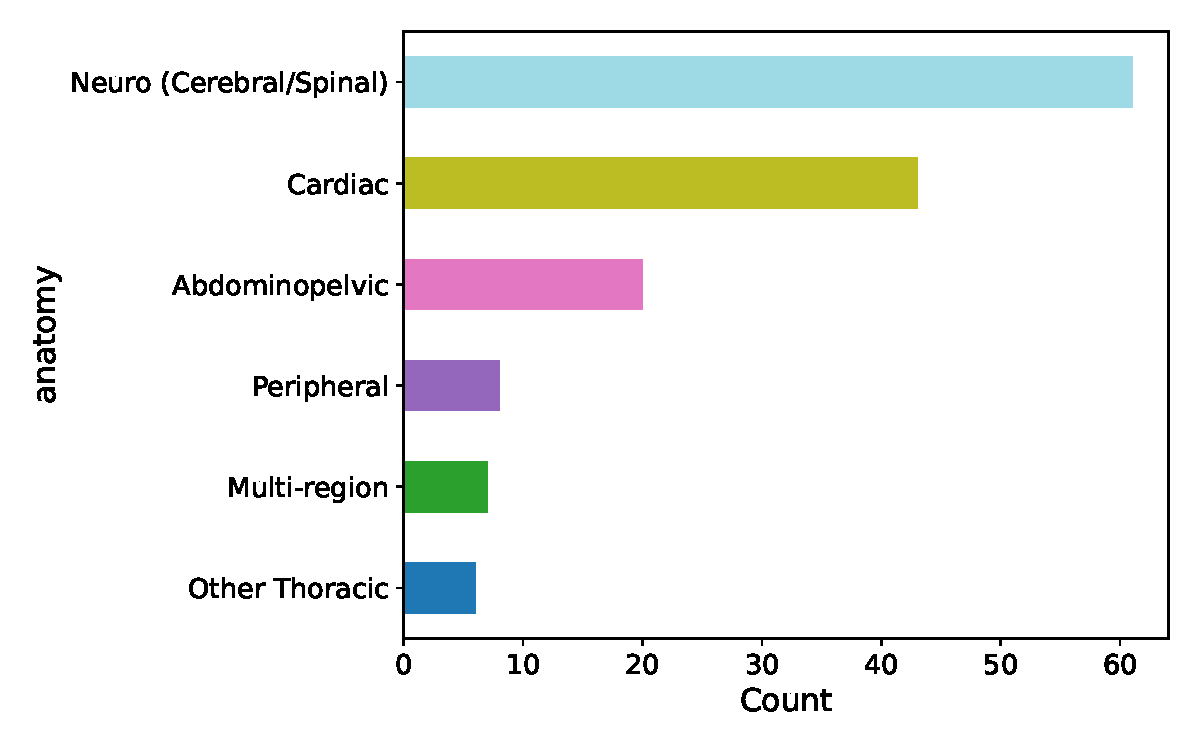
\includegraphics[width=1\linewidth]{figs/anatomy_distribution.pdf}
\caption{Territory distribution across included studies. The Neurologic category includes cerebral and spinal vascular territories.}
\label{fig:anatomy_distribution}
\end{figure}

DSA and X-ray/fluoroscopy are almost equally common (47\% and 48\% of studies; Figure~\ref{fig:modality_distribution}), but only 5 studies (4\%) use both. Cardiac (47\%) and neurologic (41\%) applications make up nearly 90\% of the corpus, while abdominopelvic, peripheral and other thoracic territories are rare (Figure~\ref{fig:anatomy_distribution}). Whether models trained on coronary or cerebral angiography transfer to other vascular beds is rarely tested.

\vspace{0.25cm}
\begin{mdframed}[linewidth=0.5pt, linecolor=black, backgroundcolor=blue!10]
\textbf{Finding 2.} Studies use DSA or X-ray/\allowbreak fluoroscopy in nearly equal numbers but almost never both, and nearly 90\% address cardiac or neurologic territories.
\end{mdframed}
\vspace{0.25cm}

\subsection{Computational Tasks and Architectures}
\label{subsec:tasks_architectures}
\begin{figure}[]
\centering
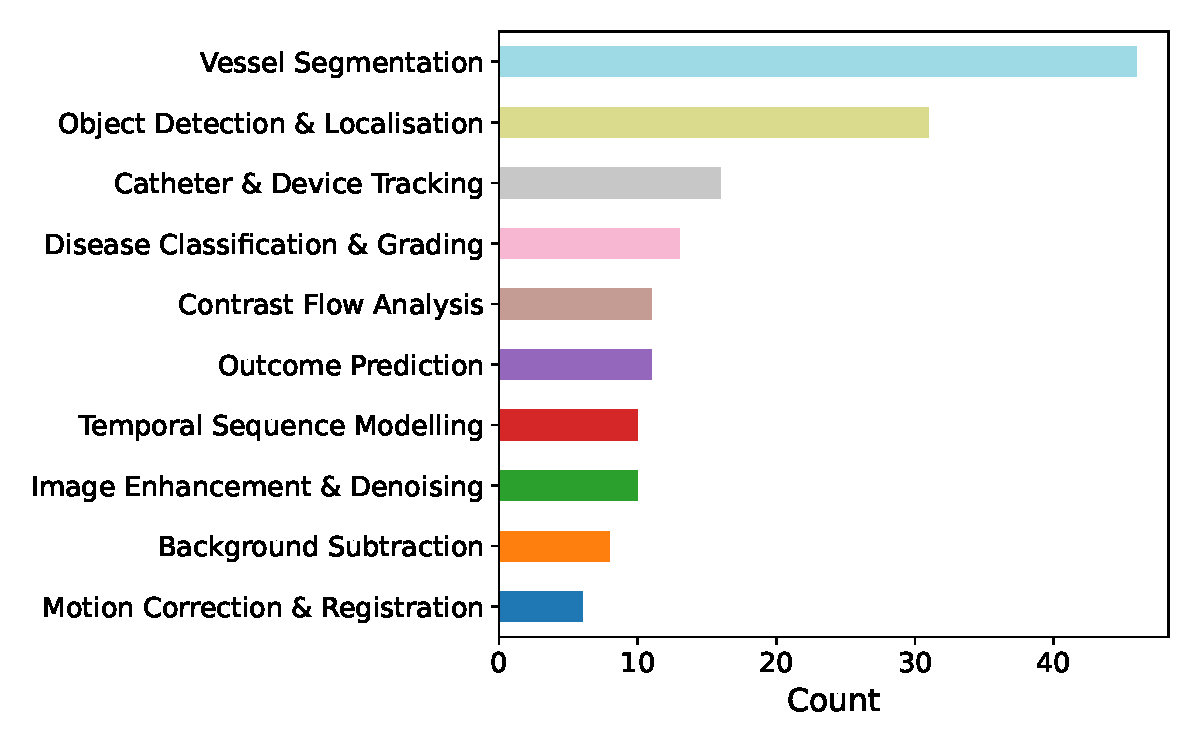
\includegraphics[width=1\linewidth]{figs/task_distribution.pdf}
\caption{Distribution of primary computational tasks across included studies.}
\label{fig:task_distribution}
\end{figure}

Disease classification and grading is the most common primary task (31 of 120 studies), followed by object detection and localization (18) and vessel segmentation (15) (Figure~\ref{fig:task_distribution}). Architectures follow the task (Table~\ref{tab:task_architecture_clean}): 14 of the 15 segmentation studies use encoder--decoder models, mostly U-Net variants; detection studies use YOLO, DETR and R-CNN detectors on ResNet backbones; classification relies on ResNet-style CNNs, with Transformers increasingly added. Most architectures are adapted from natural-image computer vision rather than designed for angiography.

Tasks whose output is itself temporal remain rare: temporal sequence modeling (6 studies) and contrast flow analysis (9). Many spatial tasks, such as segmentation, detection and classification, use several frames only to stabilize a per-frame prediction (Section~\ref{subsec:temporal_taxonomy}).

\subsubsection{Task Category Overlap}
\label{subsec:task_dendrogram}
\begin{figure}[]
\centering
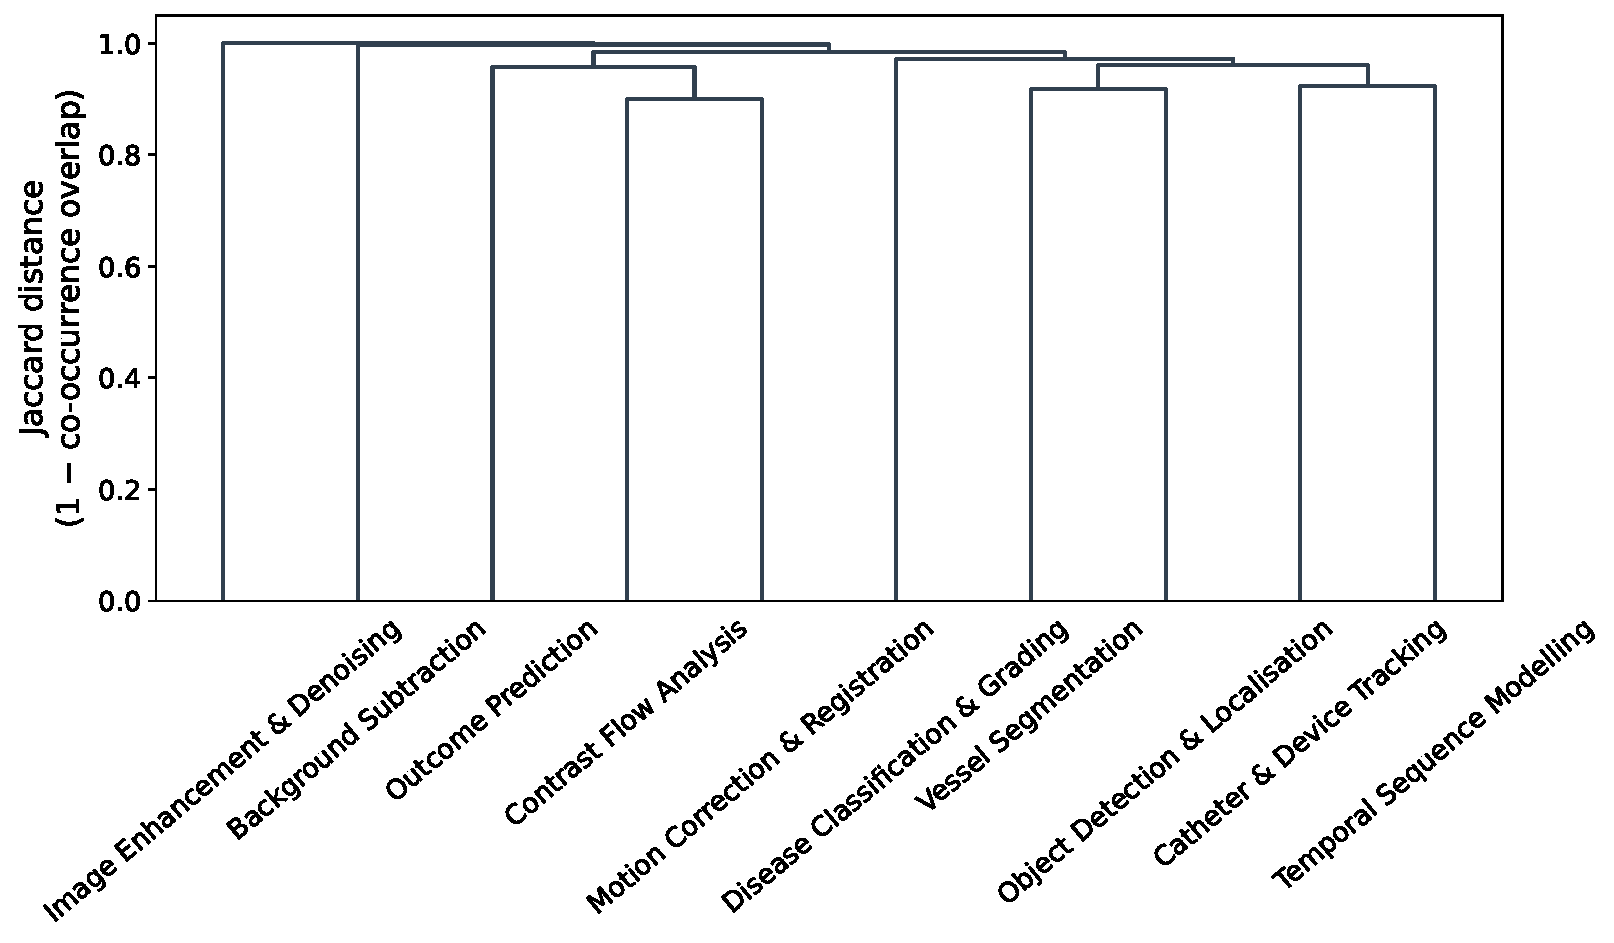
\includegraphics[width=1\linewidth]{figs/task_dendrogram.pdf}
\caption{Average-linkage (UPGMA) clustering of the ten primary task categories by Tanimoto distance between the sets of studies in each category. Merges further left mean more frequent co-occurrence. All merges fall between 0.75 and 1.00, so the axis is zoomed to that range; the two lowest sub-clusters are colored.}
\label{fig:task_dendrogram}
\end{figure}

Most task pairs merge near the maximum Tanimoto distance, so the ten categories are largely distinct (Figure~\ref{fig:task_dendrogram}). Three pairs merge earlier and are the natural candidates for a coarser taxonomy: contrast flow analysis with outcome prediction (flow measurements used as outcome predictors), classification with detection (lesions detected, then graded), and temporal sequence modeling with segmentation (vessels separated by filling phase). Image enhancement with device tracking, and motion correction with background subtraction, join the rest of the tree last.

\subsubsection{Temporal Modeling}
\label{subsec:temporal_taxonomy}
\renewcommand{\arraystretch}{1.25}
\begin{table*}[ht]
\centering
\caption{Operational taxonomy of temporal-modeling strategies, derived from the
\texttt{method.temporal\_modelling} flag and \texttt{method.temporal\_mechanism}
free-text field recorded during full-text extraction, classified via a
deterministic keyword-based rule set. N and \% are computed over the 206
records that reached full-text extraction.}
\label{tab:temporal_taxonomy}
\begin{tabularx}{\textwidth}{@{}l X r r@{}}
\toprule
\textbf{Category} & \textbf{Operational Definition} & \textbf{N} & \textbf{\%} \\
\midrule
No Temporal Use
  & Each frame (or a spatially/temporally pooled representation) is processed
    independently, with no explicit mechanism linking information across frames.
  & 129 & 62.6\% \\
\hdashline
Frame Aggregation
  & Multiple frames are combined via simple, non-learned operations (channel
    stacking, concatenation, frame differencing) before a standard 2D model.
  & 9 & 4.4\% \\
\hdashline
Optical Flow / Registration
  & Explicit frame-to-frame motion estimation, registration, or classical
    tracking/association (e.g., optical flow, particle filters,
    cross-correlation).
  & 12 & 5.8\% \\
\hdashline
RNN / LSTM / GRU
  & Recurrent architectures (LSTM, GRU, ConvLSTM, recurrent residual modules)
    propagate a hidden state across the sequence.
  & 12 & 5.8\% \\
\hdashline
3D CNN / Video Model
  & 3D or spatiotemporal convolutions, or video-/sequence-level representation
    learning, treating the sequence as a joint spatiotemporal volume.
  & 15 & 7.3\% \\
\hdashline
Transformer / State-Space
  & Self-attention or state-space mechanisms modeling long-range dependencies
    across frames.
  & 9 & 4.4\% \\
\hdashline
Hemodynamic / Physics-Informed
  & Explicit physiological or physics-based temporal modeling (reduced-order
    flow models, hemodynamic priors, physiologic signal filtering).
  & 6 & 2.9\% \\
\midrule
Not reported in extraction
  & Full-text extraction did not yield a determinable temporal-modeling
    classification for this record.
  & 14 & 6.8\% \\
\midrule
\textbf{Total} & & \textbf{206} & \textbf{100.0\%} \\
\bottomrule
\end{tabularx}
\end{table*}


Of the 120 studies, 97 (80.8\%) use an explicit mechanism that links frames, 21 (17.5\%) process frames independently, and 2 (1.7\%) do not state how frames enter the model (Table~\ref{tab:temporal_taxonomy}). The high rate partly reflects our requirement for sequence data (I2). The most common strategies are 3D/video convolution (20 studies), optical flow or registration (19) and recurrent networks (18), followed by frame aggregation (15) and hemodynamic or physics-based models (15). Transformer or state-space models are the least common (10, 8.3\%).

\renewcommand{\arraystretch}{1.2}
\begin{table*}[pos=ht]
\centering
\caption{Share of studies using explicit temporal modeling (any category in Table~\ref{tab:temporal_taxonomy} except ``No Temporal Use'') by primary task, modality and territory. Rows with fewer than 5 studies are omitted: Background Subtraction (4); Other task (1); Other modality (1); Peripheral (1); Other Thoracic (incl. aortic) (2); Multi-region (1); Not reported (1).}
\label{tab:temporal_crosstab}
\begin{tabularx}{\textwidth}{@{}X r r@{}}
\toprule
\textbf{Dimension} & \textbf{N} & \textbf{Temporal-Use Rate} \\
\midrule
\multicolumn{3}{@{}l}{\textit{By Primary Task}} \\
\dashedrule
Temporal Sequence Modelling & 6 & 100\% \\
Contrast Flow Analysis & 8 & 100\% \\
Outcome Prediction & 9 & 89\% \\
Image Enhancement \& Denoising & 9 & 89\% \\
Vessel Segmentation & 15 & 87\% \\
Disease Classification \& Grading & 29 & 83\% \\
Motion Correction \& Registration & 9 & 78\% \\
Object Detection \& Localisation & 16 & 69\% \\
Catheter \& Device Tracking & 9 & 67\% \\
\midrule
\multicolumn{3}{@{}l}{\textit{By Imaging Modality}} \\
\dashedrule
DSA & 54 & 87\% \\
X-ray / Fluoroscopy & 55 & 80\% \\
DSA + Fluoroscopy (both) & 5 & 60\% \\
\midrule
\multicolumn{3}{@{}l}{\textit{By Anatomical Territory}} \\
\dashedrule
Neurologic & 47 & 91\% \\
Cardiac & 53 & 79\% \\
Abdominopelvic & 10 & 60\% \\
\bottomrule
\end{tabularx}
\end{table*}


Adoption varies by task, from 100\% for temporal sequence modeling to 67\% for catheter and device tracking (Table~\ref{tab:temporal_crosstab}). It is higher for DSA (86\%) than for X-ray/fluoroscopy (78\%), and higher for neurologic (90\%) than for cardiac (77\%) or abdominopelvic (60\%) studies. By year, it rose from 40\% in 2018--2019 (2 of 5 studies) to 75--100\% in 2020--2025, and is 59\% (10 of 17) in the partial year 2026.

Most of this use is shallow. Of the 97 temporally aware studies, 49 rely on fixed operations (frame aggregation, optical flow or registration, hemodynamic models) and 48 (40.0\% of the corpus) learn temporal representations with recurrent, 3D/video or Transformer/state-space models. Learned models concentrate in disease classification (21 of 31 studies). They are absent from image enhancement and device tracking (0 of 9 each) and nearly absent from flow analysis and outcome prediction (1 of 9 each), the tasks whose targets are defined by temporal dynamics. Their share rose from 31.7\% of studies published in 2018--2022 (13 of 41) to 44.3\% of those published in 2023--2026 (35 of 79). Forty-one studies (34.2\%) feed a short stack of frames rather than the full sequence, and 63 studies name limited temporal modeling as a limitation (gap G3), including 51 that already model time.

\begin{table*}[t]
\centering
\small
\begin{tabularx}{\textwidth}
{>{\raggedright\arraybackslash}p{3.3cm}
 >{\raggedright\arraybackslash}X}
\toprule
\textbf{Task} & \textbf{Representative Architectures} \\
\midrule
3D Reconstruction \& Depth Estimation &
Deep Segmentation + Bi-Plane Reconstruction~ \\  % TODO(slr-122): citation(s) to studies outside the 122 removed here; claim needs re-support or rewording
\hdashline
Anomaly Detection &
Support Vector Machine, X3D Family~\cite{ref25} \\  % TODO(slr-122): citation(s) to studies outside the 122 removed here; claim needs re-support or rewording
\hdashline
Background Subtraction &
CNNs~\cite{ref52}, U-Net Family~\cite{ref40}, GAN-based Models, CDSA-Net~ \\  % TODO(slr-122): citation(s) to studies outside the 122 removed here; claim needs re-support or rewording
\hdashline
Catheter \& Device Tracking &
U-Net Family, FCN-based Networks, Vision Transformer Hybrids~\cite{ref56}, R-CNN Family, Bayesian Filtering + Siamese~\cite{ref99}, Support Vector Machine, PAR-Net~ \\  % TODO(slr-122): citation(s) to studies outside the 122 removed here; claim needs re-support or rewording
\hdashline
Contrast Flow Analysis &
CNNs~\cite{ref69}, ResNet Family, U-Net Family~\cite{ref28}, Recurrent Models (GRU)~\cite{ref96}, Physics-Informed Learning~\cite{ref43}, pix2pix, SymDIRECT~ \\  % TODO(slr-122): citation(s) to studies outside the 122 removed here; claim needs re-support or rewording
\hdashline
Disease Classification \& Grading &
ResNet Family, DenseNet Family~\cite{ref62}, EfficientNet Family~\cite{ref76}, Vision Transformer Family, X3D Family~\cite{ref25}, CVFSNet~\cite{ref35}, Faster R-CNN, Dr-SAM~ \\  % TODO(slr-122): citation(s) to studies outside the 122 removed here; claim needs re-support or rewording
\hdashline
Image Enhancement \& Denoising &
CNNs~\cite{ref10}, U-Net Family~\cite{ref39}, GAN-based Models~\cite{ref93}, Edge-Enhancement DenseNet, RED-CNN, AaDSA, EEDN~ \\  % TODO(slr-122): citation(s) to studies outside the 122 removed here; claim needs re-support or rewording
\hdashline
Image Registration &
Projective Spatial Transformers (U-Net based)~ \\  % TODO(slr-122): citation(s) to studies outside the 122 removed here; claim needs re-support or rewording
\hdashline
Landmark \& Keypoint Detection &
Hourglass-based Detection~ \\  % TODO(slr-122): citation(s) to studies outside the 122 removed here; claim needs re-support or rewording
\hdashline
Motion Correction \& Registration &
U-Net Family~\cite{ref40}, CNNs~\cite{ref96}, Projective Spatial Transformer, JTML~ \\  % TODO(slr-122): citation(s) to studies outside the 122 removed here; claim needs re-support or rewording
\hdashline
Object Detection \& Localization &
YOLO Family, Transformer Detection~\cite{ref66}, R-CNN Family, RetinaNet, ResNet Family~\cite{ref100}, DenseNet Family~\cite{ref78}, U-Net Family, Siamese Networks, Tree-based Models~ \\  % TODO(slr-122): citation(s) to studies outside the 122 removed here; claim needs re-support or rewording
\hdashline
Outcome Prediction &
Dense Neural Networks, DenseNet Family~\cite{ref42}, EfficientNet Family~\cite{ref76}, ResNet Family~\cite{ref71}, Recurrent Models~\cite{ref96}, Tree-based Models, Parametric Imaging~\cite{ref72}, SPARNet~ \\  % TODO(slr-122): citation(s) to studies outside the 122 removed here; claim needs re-support or rewording
\hdashline
Temporal Sequence Modeling &
CNNs~\cite{ref20}, ResNet Family~\cite{ref62}, Tree-based Models, Recurrent Models, Deep Channel Attention~\cite{ref97}, MoSt-DSA~\cite{ref104}, SAVE-Net~\cite{ref152}, SepConv++~\cite{ref51} \\  % TODO(slr-122): citation(s) to studies outside the 122 removed here; claim needs re-support or rewording
\hdashline
Vessel Segmentation &
U-Net Family, Temporal Attention Networks~\cite{ref64}, DenseNet Family~\cite{ref97}, nnU-Net~\cite{ref15}, CAVE~\cite{ref50}, FSTIF-UNet~\cite{ref63}, DOSTA-Net~\cite{ref64}, Channel Attention (SDAN)~\cite{ref97}, UniverSeg, DeepMedic, DFA-Net, MA-Net, MDA-Net, TAG-DL~\cite{ref56}, TBENet~ \\  % TODO(slr-122): citation(s) to studies outside the 122 removed here; claim needs re-support or rewording
\hdashline
Other &
ResNet Family~\cite{ref30}, SegFormer-style Transformer, Diffusion/Generative Models~\cite{ref39}, U-Net Family, VGG-based Models~\cite{ref94}, X3D-S~\cite{ref25}, YOLO Family, FluoroSAM, HyperMorph~\cite{ref40}, Light U-Net, RAFT~\cite{ref74}, nnU-Net+pix2pix cGAN~ \\  % TODO(slr-122): citation(s) to studies outside the 122 removed here; claim needs re-support or rewording
\bottomrule
\end{tabularx}
\caption{Task-wise mapping of representative architectural families. Architecturally similar variants (e.g., U-Net derivatives, ResNet variants, YOLO versions, and Transformer-based models) are grouped to improve readability.}
\label{tab:task_architecture_clean}
\end{table*}





% \begin{table*}[t]
% \centering
% \small
% \begin{tabularx}{\textwidth}
% {>{\raggedright\arraybackslash}p{3.3cm}
%  >{\raggedright\arraybackslash}X}
% \toprule
% \textbf{Task} & \textbf{Representative Architectures} \\
% \midrule

% 3D Reconstruction \& Depth Estimation &
% DAMN \\

% \hdashline

% Anomaly Detection &
% Support Vector Machine, X3D Family \\

% \hdashline

% Background Subtraction &
% CNNs, U-Net Family, GAN-based Models, CDSA-Net \\

% \hdashline

% Catheter \& Device Tracking &
% U-Net Family, DeepLab Family, FCN-based Networks, SegNet, Vision Transformer Hybrids, R-CNN Family, Reinforcement Learning (SAC), Support Vector Machine, Siamese Networks, PAR-Net \\

% \hdashline

% Contrast Flow Analysis &
% CNNs, ResNet Family, U-Net Family, Recurrent Models (GRU), pix2pix, SymDIRECT, Physics-ML Hybrid Models \\

% \hdashline

% Disease Classification \& Grading &
% ResNet Family, DenseNet Family, EfficientNet Family, Vision Transformer Family, X3D Family, CVFSNet, Dr-SAM, Faster R-CNN \\

% \hdashline

% Image Enhancement \& Denoising &
% CNNs, U-Net Family, GAN-based Models, Dense DnCNN, RED-CNN, AaDSA, EEDN \\

% \hdashline

% Image Registration &
% U-Net Family \\

% \hdashline

% Landmark \& Keypoint Detection &
% SA-Hourglass \\

% \hdashline

% Motion Correction \& Registration &
% U-Net Family, CNNs, JTML, ProST DeepNet \\

% \hdashline

% Object Detection \& Localization &
% YOLO Family, DETR Family, R-CNN Family, RetinaNet, ResNet Family, Vision Transformer Family, DenseNet Family, U-Net Family, Siamese Networks, Tree-based Models \\

% \hdashline

% Outcome Prediction &
% Dense Neural Networks, DenseNet Family, EfficientNet Family, ResNet Family, Recurrent Models, Tree-based Models, Hybrid Transformer-UNet Models, SPARNet \\

% \hdashline

% Temporal Sequence Modeling &
% CNNs, ResNet Family, Tree-based Models, Recurrent Models, MoStNet, MoSt-DSA, SAVE-Net, SepConv++ \\

% \hdashline

% Vessel Segmentation &
% U-Net Family, DeepLab Family, FCN-based Segmentation Networks, DenseNet Family, Vision Transformer Segmentation Models, nnU-Net, UniverSeg, DeepMedic, CAVE, DFA-Net, MA-Net, MDA-Net, TAG-DL, TBENet, SDAN \\

% \hdashline

% Other &
% FluoroSAM, HyperMorph, Light U-Net, RAFT, ResNet Family, SegFormer, Diffusion Models, U-Net Family, VGG-based Models, X3D-S, YOLO Family, nnU-Net+pix2pix cGAN \\

% \bottomrule
% \end{tabularx}
% \caption{Task-wise mapping of representative architectural families. Architecturally similar variants (e.g., U-Net derivatives, ResNet variants, YOLO versions, and Transformer-based models) are grouped to improve readability.}
% \label{tab:task_architecture_clean}
% \end{table*}

\vspace{0.25cm}
\begin{mdframed}[linewidth=0.5pt, linecolor=black, backgroundcolor=blue!10]
\textbf{Finding 3.} The question is how, not whether, time is modeled. 80.8\% of studies use temporal information, but half of them through fixed operations; learned sequence models cluster in classification, and Transformer or state-space models (8.3\%) all date from 2023 onward.
\end{mdframed}
\vspace{0.25cm}

\subsection{Publication Venues}
\label{subsec:venues}
\begin{figure}[]
\centering
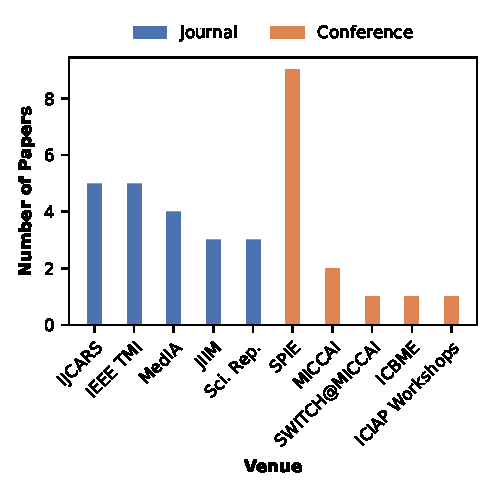
\includegraphics[width=1\linewidth]{figs/venue_analysis_stacked.pdf}
\caption{Top publication venues by paper count, stratified by venue type. IJCARS: International Journal of Computer Assisted Radiology and Surgery; IEEE TMI: IEEE Transactions on Medical Imaging; MedIA: Medical Image Analysis; JIIM: Journal of Imaging Informatics in Medicine; Sci.\ Rep.: Scientific Reports; SPIE: Proceedings of SPIE; MICCAI: International Conference on Medical Image Computing and Computer-Assisted Intervention; SWITCH@MICCAI: SWITCH workshop at MICCAI; ICBME: Iranian Conference on Biomedical Engineering; JACC: Journal of the American College of Cardiology.}
\label{fig:venue_stacked}
\end{figure}
\begin{figure}[]
\centering
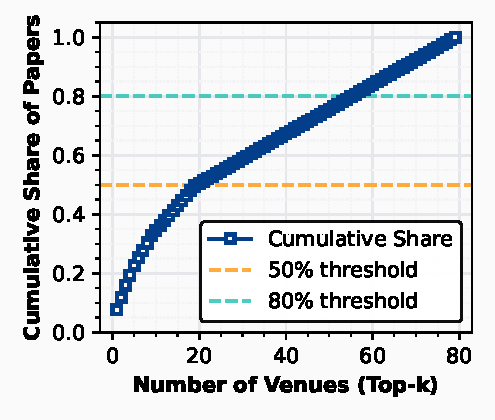
\includegraphics[width=1\linewidth]{figs/venue_cumulative_curve.pdf}
\caption{Cumulative share of studies across venues, ranked by study count. Dashed lines mark 50\% (yellow) and 80\% (green).}
\label{fig:venue_curve}
\end{figure}

Most studies are journal articles (89 of 120), with 24 conference papers and 7 preprints. The most frequent outlet is the SPIE proceedings (11 studies, 9 of them under the series name shown in Figure~\ref{fig:venue_stacked}), followed by IJCARS and IEEE TMI (5 each) and Medical Image Analysis (4). Among the 119 studies with a stated venue, half are spread across 20 venues, 56 of the 79 venues are needed to reach 80\%, and 60 venues contribute a single study (Figure~\ref{fig:venue_curve}). Engineering venues are well represented (11 studies in IEEE venues and 11 in SPIE proceedings), but MICCAI (three records) and ACM venues (none) are not, and conferences contribute far less here than in medical image computing generally.

\vspace{0.25cm}
\begin{mdframed}[linewidth=0.5pt, linecolor=black, backgroundcolor=blue!10]
\textbf{Finding 4.} No venue serves as a hub: the 120 studies are spread over 79 venues, 60 of which contribute a single study, so syntheses must search broadly.
\end{mdframed}
\vspace{0.25cm}

\subsection{Reported Performance}
\label{subsec:performance}
\begin{figure}[]
\centering
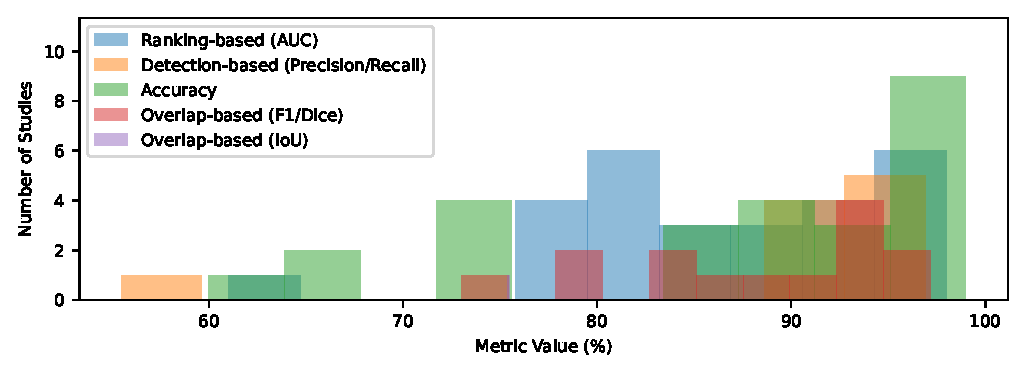
\includegraphics[width=1\linewidth]{figs/histogram_metrics.pdf}
\caption{Distribution of reported performance values by metric family.}
\label{fig:metric_histogram}
\end{figure}
\begin{figure}[]
\centering
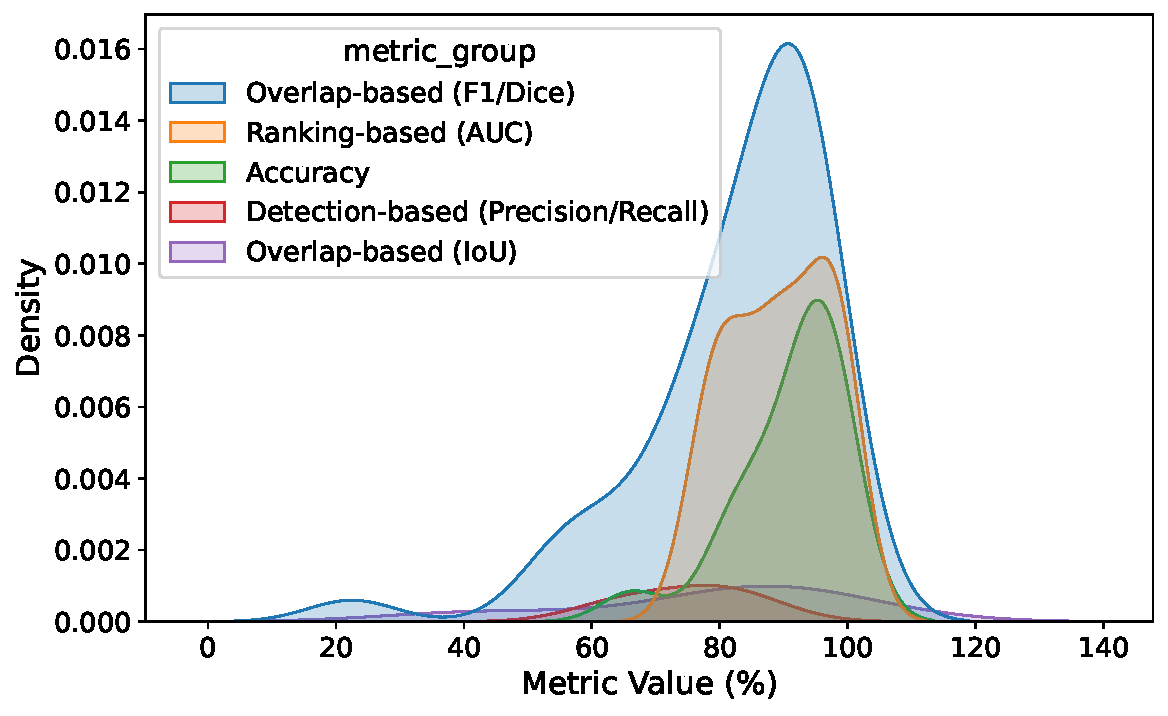
\includegraphics[width=1\linewidth]{figs/kde_metrics.pdf}
\caption{Kernel density estimates of reported performance values by metric family.}
\label{fig:metric_kde}
\end{figure}

Reported values are high in the four metric families used by more than one study, with family means between 86.6 and 89.9 on a 0--100 scale (Figures~\ref{fig:metric_histogram} and \ref{fig:metric_kde}). Accuracy (26 studies; SD 12.0, range 60--99) and detection precision and recall (10 studies; SD 12.5) are the most dispersed; Dice/F1 (14 studies; SD 7.5, range 73--97) and AUC (27 studies; SD 8.7) are tighter. Accuracy is also the least informative of these under the class imbalance common in angiographic tasks. With different datasets and protocols and no shared benchmark, these values cannot be compared across studies; the skew toward high values is consistent with publication bias and with testing on data similar to the training data.

\vspace{0.25cm}
\begin{mdframed}[linewidth=0.5pt, linecolor=black, backgroundcolor=blue!10]
\textbf{Finding 5.} Reported performance is consistently high but not comparable across studies, because datasets, protocols and metrics differ and no shared benchmark exists.
\end{mdframed}
\vspace{0.25cm}

\subsection{Reporting Quality and Clinical Readiness}
\label{subsec:reporting_quality}
\begin{figure*}[]
\centering
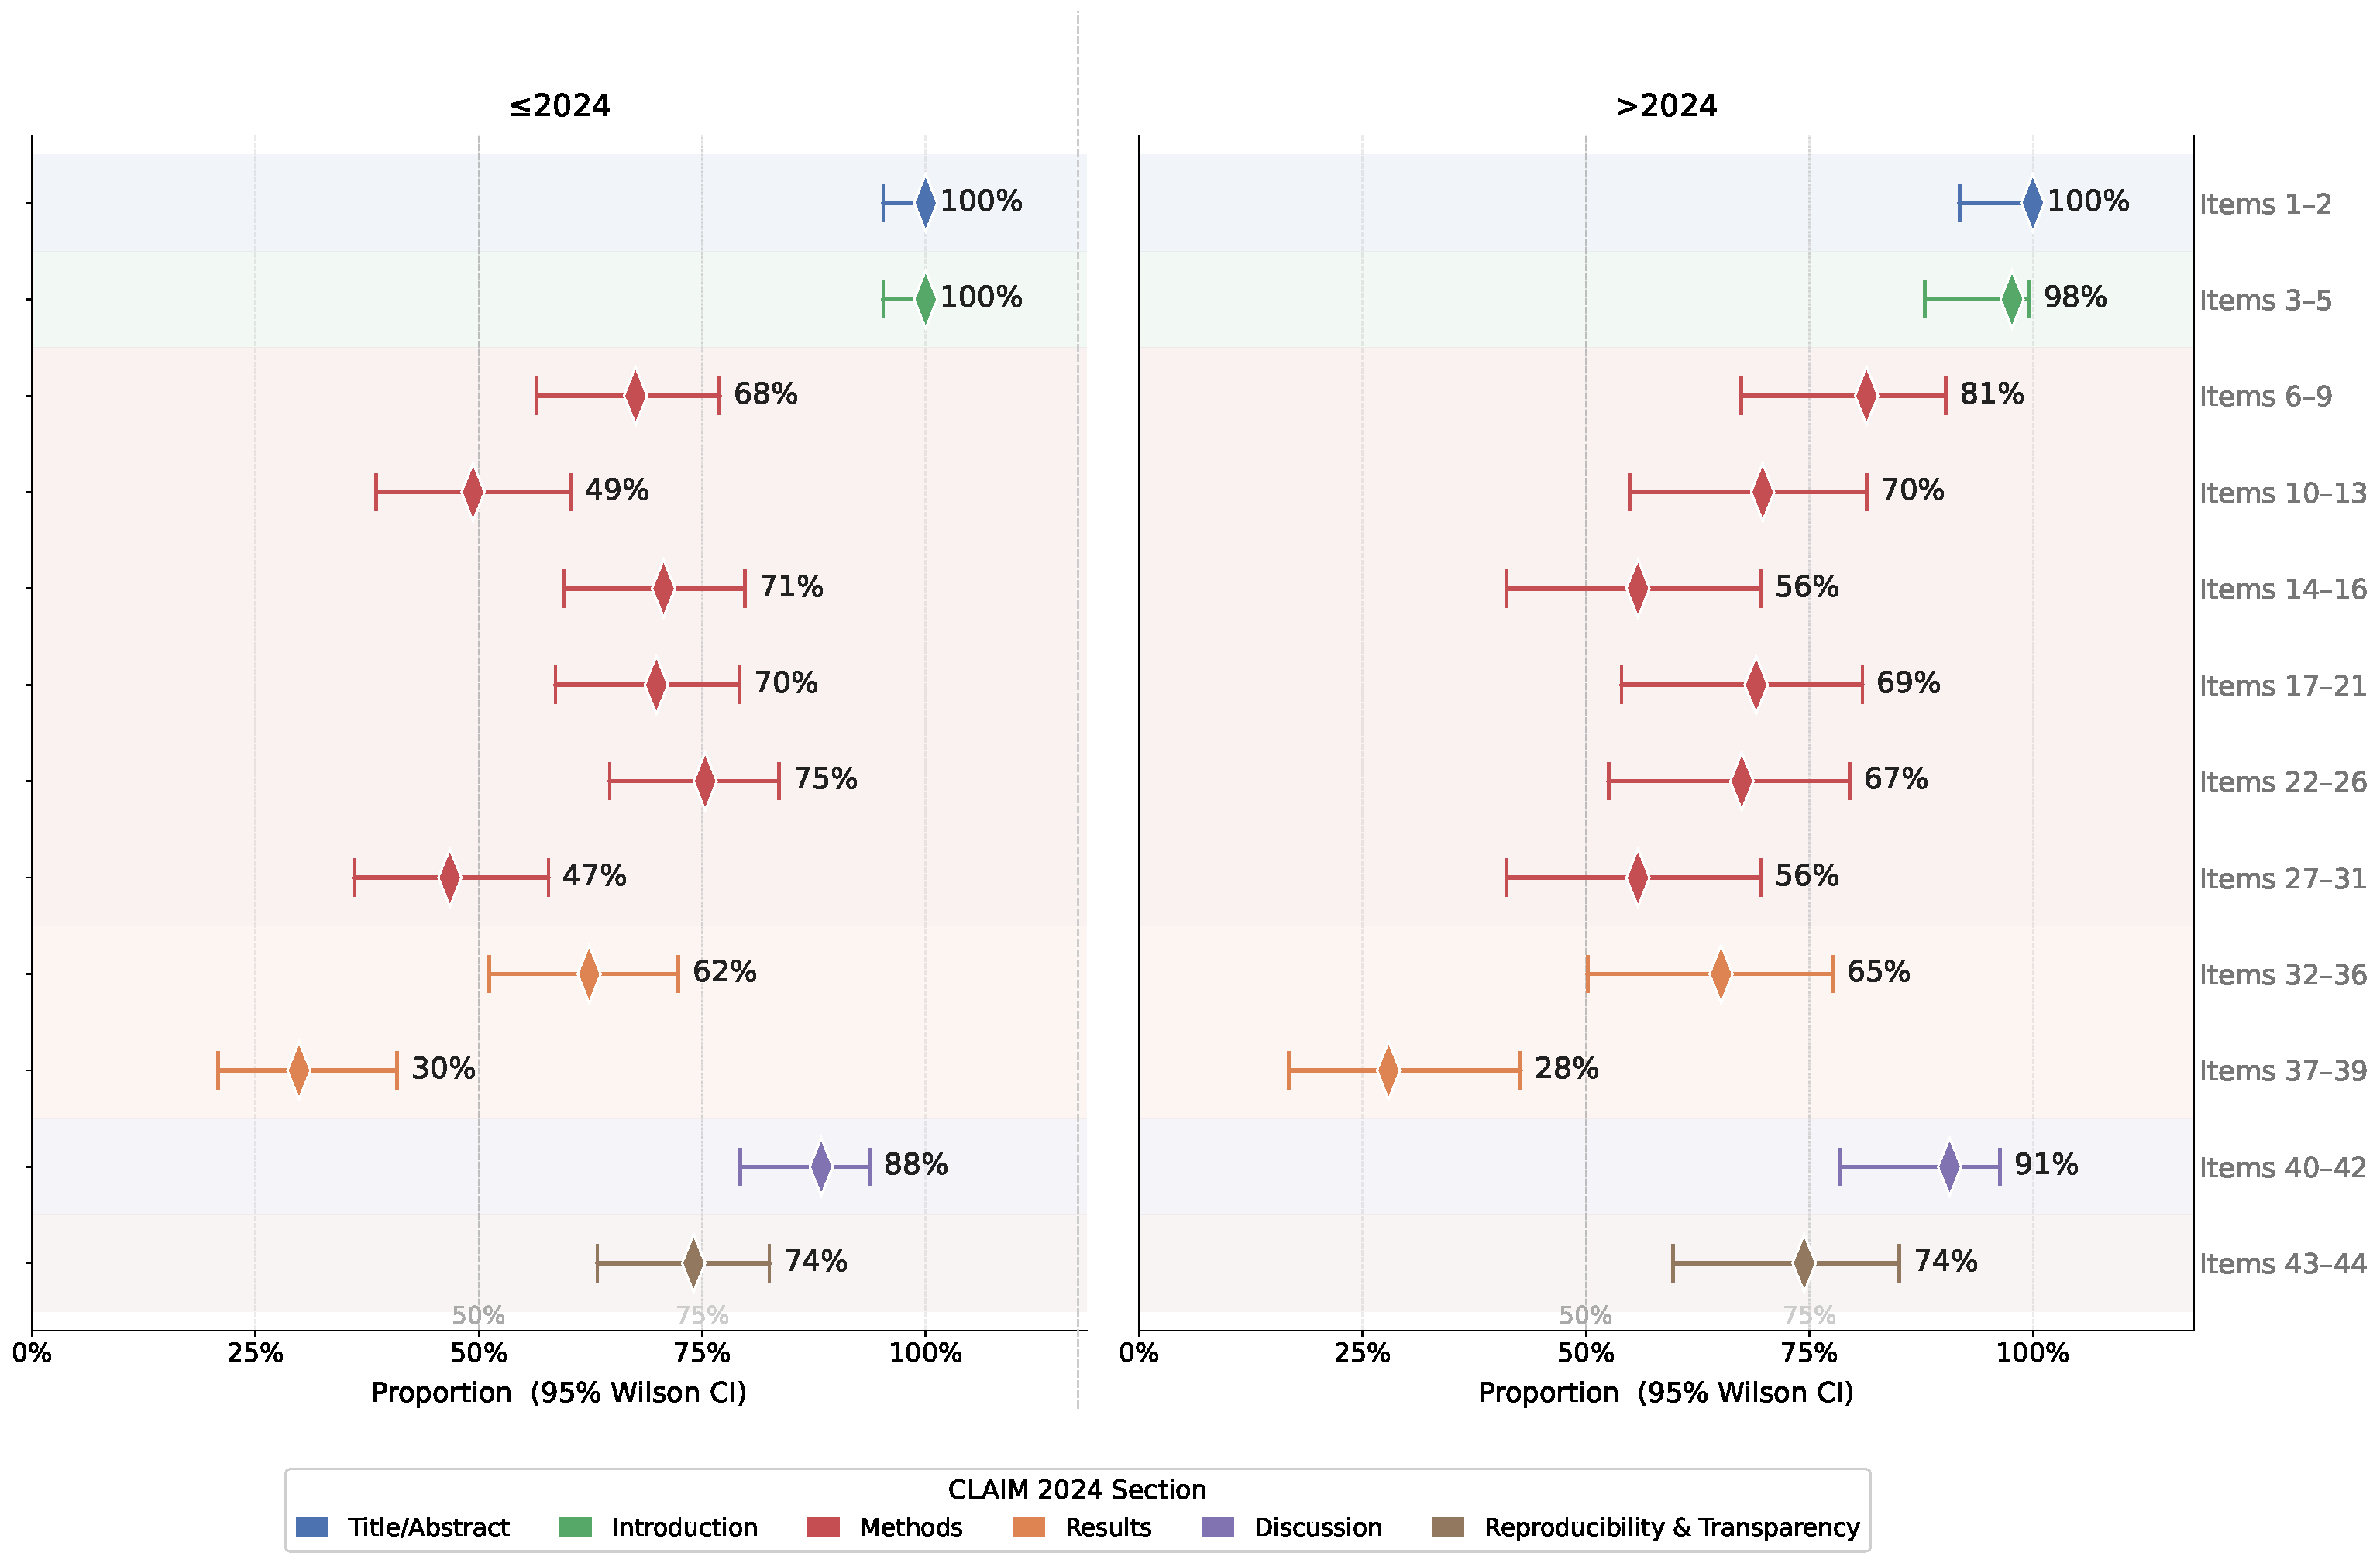
\includegraphics[width=1\linewidth]{figs/forest_plot_claim2024_comparison.pdf}
\caption{CLAIM 2024 adherence by cluster for studies published up to 2024 (left) and from 2025 onward (right). Diamonds show the proportion of studies meeting each cluster, with 95\% Wilson confidence intervals; colors mark the CLAIM section, and the right axis lists the checklist items in each cluster~\cite{Tejani2024}.}
\label{fig:forest_plot}
\end{figure*}

\definecolor{claimTA}{HTML}{4C72B0}
\definecolor{claimIntro}{HTML}{55A868}
\definecolor{claimMeth}{HTML}{C44E52}
\definecolor{claimRes}{HTML}{DD8452}
\definecolor{claimDisc}{HTML}{8172B2}
\definecolor{claimRepro}{HTML}{937860}

\begin{table}[ht]
  \centering
  \caption{CLAIM 2024 Adherence by Thematic Cluster: Temporal Comparison
    ($\leq 2024$ vs.\ $\geq 2025$).}
  \label{tab:claim2024_temporal}

  \footnotesize
  \renewcommand{\arraystretch}{1.25}
  \setlength{\tabcolsep}{4pt}

  \resizebox{\columnwidth}{!}{%
  \begin{tabular}{@{}
      l
      p{6.2cm}
      r r
      r r
      >{\centering\arraybackslash}p{1.2cm}
  @{}}

    \toprule

    \multicolumn{1}{l}{\textbf{ID}} &
    \multicolumn{1}{l}{\textbf{Cluster}} &
    \multicolumn{2}{c}{$\boldsymbol{\leq 2024}$ \textbf{(N\,=\,127)}} &
    \multicolumn{2}{c}{$\boldsymbol{\geq 2025}$ \textbf{(N\,=\,56)}} &
    \multicolumn{1}{c}{$\boldsymbol{\Delta}$} \\

    \cmidrule(lr){3-4}
    \cmidrule(lr){5-6}

    & &
    \textbf{\%} & \textbf{95\% CI} &
    \textbf{\%} & \textbf{95\% CI} &
    \\

    \midrule

    \rowcolor{claimTA!15}
    \multicolumn{7}{l}{\textbf{\textcolor{claimTA}{Title/Abstract}}} \\

    C01 & AI identification \& abstract completeness
    & 71\% & [62, 78]
    & 75\% & [62, 84]
    & $+4\%$~$\uparrow$ \\

    \midrule

    \rowcolor{claimIntro!15}
    \multicolumn{7}{l}{\textbf{\textcolor{claimIntro}{Introduction}}} \\

    C02 & Background \& study objectives
    & 98\% & [94, 100]
    & 98\% & [91, 100]
    & $\pm0\%$~$\sim$ \\

    \midrule

    \rowcolor{claimMeth!15}
    \multicolumn{7}{l}{\textbf{\textcolor{claimMeth}{Methods}}} \\

    C03 & Study design \& data sources
    & 42\% & [34, 50]
    & 61\% & [48, 72]
    & $+19\%$~$\uparrow$ \\

    C04 & Participants \& image acquisition
    & 29\% & [21, 37]
    & 38\% & [26, 51]
    & $+9\%$~$\uparrow$ \\

    C05 & Ground truth \& annotation
    & 31\% & [24, 40]
    & 46\% & [34, 59]
    & $+15\%$~$\uparrow$ \\

    C06 & Data partitioning \& class handling
    & 44\% & [36, 53]
    & 44\% & [31, 57]
    & $\pm0\%$~$\sim$ \\

    C07 & Model architecture \& training
    & 65\% & [56, 72]
    & 64\% & [50, 75]
    & $-1\%$~$\sim$ \\

    C08 & Evaluation design \& fairness
    & 24\% & [17, 32]
    & 52\% & [39, 64]
    & $+28\%$~$\uparrow$ \\

    \midrule

    \rowcolor{claimRes!15}
    \multicolumn{7}{l}{\textbf{\textcolor{claimRes}{Results}}} \\

    C09 & Performance \& external validation
    & 35\% & [27, 44]
    & 44\% & [31, 57]
    & $+9\%$~$\uparrow$ \\

    C10 & Demographic \& subgroup reporting
    & 8\% & [4, 14]
    & 16\% & [9, 28]
    & $+8\%$~$\uparrow$ \\

    \midrule

    \rowcolor{claimDisc!15}
    \multicolumn{7}{l}{\textbf{\textcolor{claimDisc}{Discussion}}} \\

    C11 & Limitations, implications \& future work
    & 84\% & [77, 90]
    & 89\% & [79, 95]
    & $+5\%$~$\uparrow$ \\

    \midrule

    \rowcolor{claimRepro!15}
    \multicolumn{7}{l}{\textbf{\textcolor{claimRepro}{Reproducibility \& Transparency}}} \\

    C12 & Reproducibility \& funding disclosure
    & 21\% & [15, 29]
    & 23\% & [14, 36]
    & $+2\%$~$\sim$ \\

    \bottomrule

    \multicolumn{7}{p{\hsize}}{%
      \textit{Note:} Proportions are the fraction of studies reporting adherence
      (``Yes'') among those where the item was applicable (NA excluded).
      95\% Wilson confidence intervals are shown.
      $\Delta$ = post--pre difference; arrows indicate changes greater than
      2 percentage points.
    } \\

  \end{tabular}%
  }

\end{table}
% \definecolor{claimTA}{HTML}{4C72B0}
% \definecolor{claimIntro}{HTML}{55A868}
% \definecolor{claimMeth}{HTML}{C44E52}
% \definecolor{claimRes}{HTML}{DD8452}
% \definecolor{claimDisc}{HTML}{8172B2}
% \definecolor{claimRepro}{HTML}{937860}

% \begin{table}[ht]
%   \centering
%   \caption{CLAIM 2024 Adherence by Thematic Cluster: Temporal Comparison
%     ($\leq 2024$ vs.\ $\geq 2025$).}
%   \label{tab:claim2024_temporal}

%   \footnotesize
%   \renewcommand{\arraystretch}{1.25}
%   \setlength{\tabcolsep}{4pt}

%   \resizebox{\columnwidth}{!}{%
%   \begin{tabular}{@{}
%       l
%       p{6.2cm}
%       r r
%       r r
%       >{\centering\arraybackslash}p{1.2cm}
%   @{}}

%     \toprule

%     \multicolumn{1}{l}{\textbf{ID}} &
%     \multicolumn{1}{l}{\textbf{Cluster}} &
%     \multicolumn{2}{c}{$\boldsymbol{\leq 2024}$ \textbf{(N\,=\,127)}} &
%     \multicolumn{2}{c}{$\boldsymbol{\geq 2025}$ \textbf{(N\,=\,56)}} &
%     \multicolumn{1}{c}{$\boldsymbol{\Delta}$} \\

%     \cmidrule(lr){3-4}
%     \cmidrule(lr){5-6}

%     & &
%     \textbf{\%} & \textbf{95\% CI} &
%     \textbf{\%} & \textbf{95\% CI} &
%     \\

%     \midrule

%     \rowcolor{claimTA!15}
%     \multicolumn{7}{l}{\textbf{\textcolor{claimTA}{Title/Abstract}}} \\

%     C01 & AI identification \& abstract completeness
%     & 71\% & [62, 78]
%     & 75\% & [62, 84]
%     & $+4\%$~$\uparrow$ \\

%     \midrule

%     \rowcolor{claimIntro!15}
%     \multicolumn{7}{l}{\textbf{\textcolor{claimIntro}{Introduction}}} \\

%     C02 & Background \& study objectives
%     & 98\% & [94, 100]
%     & 98\% & [91, 100]
%     & $\pm0\%$~$\sim$ \\

%     \midrule

%     \rowcolor{claimMeth!15}
%     \multicolumn{7}{l}{\textbf{\textcolor{claimMeth}{Methods}}} \\

%     C03 & Study design \& data sources
%     & 42\% & [34, 50]
%     & 61\% & [48, 72]
%     & $+19\%$~$\uparrow$ \\

%     C04 & Participants \& image acquisition
%     & 29\% & [21, 37]
%     & 38\% & [26, 51]
%     & $+9\%$~$\uparrow$ \\

%     C05 & Ground truth \& annotation
%     & 31\% & [24, 40]
%     & 46\% & [34, 59]
%     & $+15\%$~$\uparrow$ \\

%     C06 & Data partitioning \& class handling
%     & 44\% & [36, 53]
%     & 44\% & [31, 57]
%     & $\pm0\%$~$\sim$ \\

%     C07 & Model architecture \& training
%     & 65\% & [56, 72]
%     & 64\% & [50, 75]
%     & $-1\%$~$\sim$ \\

%     C08 & Evaluation design \& fairness
%     & 24\% & [17, 32]
%     & 52\% & [39, 64]
%     & $+28\%$~$\uparrow$ \\

%     \midrule

%     \rowcolor{claimRes!15}
%     \multicolumn{7}{l}{\textbf{\textcolor{claimRes}{Results}}} \\

%     C09 & Performance \& external validation
%     & 35\% & [27, 44]
%     & 44\% & [31, 57]
%     & $+9\%$~$\uparrow$ \\

%     C10 & Demographic \& subgroup reporting
%     & 8\% & [4, 14]
%     & 16\% & [9, 28]
%     & $+8\%$~$\uparrow$ \\

%     \midrule

%     \rowcolor{claimDisc!15}
%     \multicolumn{7}{l}{\textbf{\textcolor{claimDisc}{Discussion}}} \\

%     C11 & Limitations, implications \& future work
%     & 84\% & [77, 90]
%     & 89\% & [79, 95]
%     & $+5\%$~$\uparrow$ \\

%     \midrule

%     \rowcolor{claimRepro!15}
%     \multicolumn{7}{l}{\textbf{\textcolor{claimRepro}{Reproducibility \& Transparency}}} \\

%     C12 & Reproducibility \& funding disclosure
%     & 21\% & [15, 29]
%     & 23\% & [14, 36]
%     & $+2\%$~$\sim$ \\

%     \bottomrule

%     \multicolumn{7}{p{\hsize}}{%
%       \textit{Note:} Proportions are the fraction of studies reporting adherence
%       (``Yes'') among those where the item was applicable (NA excluded).
%       95\% Wilson confidence intervals are shown.
%       $\Delta$ = post--pre difference; arrows indicate changes greater than
%       2 percentage points.
%     } \\

%   \end{tabular}%
%   }

% \end{table}


We assessed all 120 studies against CLAIM 2024~\cite{Tejani2024}, the RSNA reporting checklist for AI in medical imaging (Figure~\ref{fig:forest_plot}, Table~\ref{tab:claim2024_temporal}). Background and objectives are reported almost universally; methods reporting is weaker and uneven. Between studies published up to 2024 and those from 2025 onward, the largest differences are in participant and image-acquisition reporting (C04: 49\% to 70\%, $p=0.04$), study design and data sources (C03: 68\% to 81\%, $p=0.14$) and ground-truth and annotation reporting, which declines (C05: 71\% to 56\%, $p=0.11$). Demographic and subgroup reporting stays low (C10: 30\% and 28\%). No difference remains significant after Holm correction (smallest adjusted $p=0.43$); with 43 recent studies, only large shifts would be detectable. Only 25 studies (20.8\%) share code and 3 (2.5\%) share data, although the reproducibility cluster (C12), which also counts funding disclosure, is met by 74\%. Evidence of clinical readiness is also thin: 19 studies (15.8\%) report external validation (one of them alongside a prospective deployment), 3 (2.5\%) a prospective design, 4 (3.3\%) clinical deployment or live use, and 4 (3.3\%) discuss regulatory requirements.

\vspace{0.25cm}
\begin{mdframed}[linewidth=0.5pt, linecolor=black, backgroundcolor=blue!10]
\textbf{Finding 6.} Reporting is strong for background and objectives but weak for subgroup analysis, code and data sharing, and has not changed measurably since CLAIM 2024.
\end{mdframed}
\vspace{0.25cm}
